\addcontentsline{toc}{chapter}{Appendices}
\chapter{Facial Feature Localisation}
\section{Gabor Filter}
2D Gabor filters which are already widely used in Texture segmentation \cite{Dunn1995} and iris recognition \cite{Daugman1993}, were proposed by J. Daugman \cite{Daugman1985}. Gabor filters are similar to the 2D receptive fields in simple cells of the mammalian cortex \cite{Jones1987}, so that modeling the Gabor filter is analogy to simulate the mammalian visual systems, which may help for accomplishing the machine vision task. Gabor filters are the particular case of joint spatial/frequency filters. Objects can be modeled in the response of Gabor filters, because Gabor filter varies in different frequencies and different orientations, which leads to the coarse-fine analysis. In face recognition, human face is such a pattern that contains the stimulus in different frequencies and different orientations. Therefore, Gabor filters can be used in face recognition.

Gabor filters are derived from Gabor elementary functions. The kernels look like Fourier basis elements that are multiplied by Gaussian. The 2D Gabor function is defined as.
\begin{equation}\label{eq:2DGaborfunction}
 H(x,y) = \frac{1}{2\pi\sigma_x\sigma_y}e^{-\frac{1}{2}[(\frac{x-x_0}{\sigma_x})^2+(\frac{y-y_0}{\sigma_y})^2]}e^{j2\pi(Ux+Vy)}
\end{equation}
where $\sigma_x$ and $\sigma_y$ characterise the standard derivations corresponding to $x$ and $y$ axis in 2D Gaussian. The parameters $(U, V)$ represent the particular 2D frequency of sinusoidal function along x and y axes. It also can be represented as a Covariance matrix
\begin{displaymath}
 \mathbf{C} = \left( \begin{array}{cc}
             \sigma_x^2 & 0 \\
	     0 & \sigma_y^2 \\
            \end{array} \right)
\end{displaymath}
The 2D Gabor filter is centred at $(x_0,y_0)$. The left part of \mbox{Equation} \ref{eq:2DGaborfunction} is a Gaussian centred at $(x_0, y_0)$ with the standard derivations $\sigma_x$ and $\sigma_y$. The right part is a complex formula. The Gabor functions are sinusoidally modulated Gaussian functions. It can be represented in pairs, often referred to as \textit{quadrature pairs} as 
\begin{displaymath}
\begin{array}{l}
 H_{\mathrm{even}} = \frac{1}{2\pi\sigma_x\sigma_y}e^{-\frac{1}{2}[(\frac{x-x_0}{\sigma_x})^2+(\frac{y-y_0}{\sigma_y})^2]} \times \cos{[2\pi(Ux+Vy)]} \\
 H_{\mathrm{odd}} = \frac{1}{2\pi\sigma_x\sigma_y}e^{-\frac{1}{2}[(\frac{x-x_0}{\sigma_x})^2+(\frac{y-y_0}{\sigma_y})^2]} \times \sin{[2\pi(Ux+Vy)]} 
\end{array}
\end{displaymath}
Just like normal complex number, the top one is called the real part, or called even part. The bottom one is called the imaginary part, or called odd part. The real part is a Gaussian modulated with a cosine function, so that it resides in a symmetric structure, because the standard cosine function (no dilation and no translation) is symmetric from $-\frac{\pi}{2}$ to $\frac{\pi}{2}$. The imaginary part is modulated with a sine function, so that it has an antisymmetric structure, because the standard sine functions are increasing monotony from $-\frac{\pi}{2}$ to $\frac{\pi}{2}$.

The 2D frequencies of sinusoidal function along $x$ and $y$ axes are specified by $(U,V)$. The complex exponential is a 2D complex sinusoid at the radial frequency $F=\sqrt{U^2+V^2}$. The different frequency combinations along $x$ and $y$ axes construct the different orientations of the sinusoid. The angle of orientation specified by
\begin{equation}
 \theta =\tan^{-1}\frac{U}{V}
\end{equation}

In most cases, the equal standard derivation in both axes $\sigma_x=\sigma_y=\sigma$ is a reasonable design choice. Normally, when a texture image contains texture pixels which are arranged in a square lattice, the symmetric filters ($\sigma_x=\sigma_y$) are useful. In addition, it is assumed that $(x_0,y_0)$ is set as the origin $(0,0)$. Hence, the Gabor function are simplified to
\begin{equation}
 h(x,y) = \frac{1}{2\pi\sigma^2} e^{-\frac{x^2+y^2}{2\sigma^2}} e^{j2\pi(Ux+Vy)}
\end{equation}
where, the parameter $\sigma$ is the deviation of 2D Gaussian which controls the size of Gaussian plot. The Gabor filter is
\begin{equation}
 m(x,y) = i(x,y)\ast h(x,y)
\end{equation}
The operator $\ast$ specifies the convolution given by
\begin{equation}
 i(x,y)\ast h(x,y) = \int \int i(u,v)j(x-u,y-v)dxdy
\end{equation}
where $i(x,y)$ is an image and $m(x,y)$ is the output which is the result of the image $i(x,y)$ convolved with the Gabor function $h(x,y)$. Because the Gabor function has complex structure, the output of filter also is in a complex structure. There are two components $m_{\mathrm{even}}(x,y)$ and $m_{\mathrm{odd}}(x,y)$ in the output $m(x,y)$. One is the image $i(x,y)$ only convolved with the real (even) kernel
\begin{displaymath}
 m_{\mathrm{even}}(x,y) = i(x,y) \ast h_{\mathrm{even}}(x,y)
\end{displaymath}
Another one is $i(x, y)$ convolved with the imaginary (odd) kernel
\begin{displaymath}
 m_{\mathrm{odd}}(x,y) = i(x,y) \ast h_{\mathrm{odd}}(x,y)
\end{displaymath}
The magnitude response is obtained from the even and odd outputs (responses), as follows.
\begin{displaymath}
 m_{\mathrm{mag}}(x,y) = \|m(x,y)\| = \sqrt{m_{\mathrm{even}}^2(x,y) + m_{\mathrm{odd}}^2(x,y)}
\end{displaymath}
The phase response is as
\begin{displaymath}
 m_{\mathrm{pha}}(x,y) = \tan^{-1}\frac{m_{\mathrm{odd}}(x,y)}{m_{\mathrm{even}}(x,y)}
\end{displaymath}

Some experiments \cite{Kruger2000} use the even responses (output) of filtering, some other use odd responses. For most Gabor filter application like texture segmentation or edge detection, the magnitude responses are used. The phase responses are not commonly used in computer vision and image processing, because it changes dramatically over an image and does not give any meaningful interpretation. In the thesis, the magnitude response is taken into account.

\section{k-Means Clustering Algorithm}
A useful phenomenon is found, which is that the high responses applied by Gabor approach look like some clusters plotting. After applied the Gabor filters on face image, the response shows some high responses always concentrate in some areas on the face, such as the eyes, the nose and the mouth. In the response images, each pixel can be considered as a point with an individual value in a two-dimensional coordination. The larger the value, the higher the response in this pixel. Most high responses are concentrated in four clusters. These four clusters are corresponding to the areas of two eyes, nose and mouth. From this clue, the facial features can be located by using some automatic clustering algorithms.

The $k$-means \cite{Alsabti1998} approach is adopted for clustering the pixels into couples of groups. Clustering is the process of partitioning or grouping a given set of examples into disjoint clusters. This is done such that examples in the same cluster are alike, and examples belonging to two different clusters are different. Clustering has been a widely studied problem in a variety of application domains including neural networks, AI, and statistics. The $k$-means method has been shown to be effective in producing good clustering results for many practical applications among some cluster algorithms. In $k$-means algorithm, the number of clusters $k$ is determined before the clustering, which means before the implementation, the number of clusters in the existing examples is known. In this way, $k$-means is not a complete solution for data clustering (some extension of $k$-means called $X$-means \cite{Pelleg2000} can estimate $k$). However, some prior knowledge of human faces is acquired, for instance, there are some clusters corresponding to eyes, nose and mouth. By using our prior knowledge on human faces, the number of clusters $k$ can be determined beforehand.

Let the $k$ prototypes $(\omega_1,\omega_2,\ldots,\omega_k)$ be initialised to one of the $n$ input examples $(i_1,i_2,\ldots,i_n)$. In this case, $n$ is the number of pixels which has the higher response. Each example $i_l$ is equal to one of the prototypes $\omega_j$. The condition is $k\ll n$, because the number of prototypes must be greatly less than the number of input examples, so that the clustering algorithm can be effective, also assuming that well defined clusters exist. The principle of $k$-means algorithm is to assign each example to different cluster, and give the prototypes that are also the centroids of clusters.  In $n$ input examples, there may be $k$ clusters. $C_j$ represents the $j$th ($0<j\le k$) cluster whose value is a disjoint subset of input examples.

The $k$-means algorithm is described as \mbox{Table} \ref{tab:kmeans}. For an individual example, the best prototype should have the minimum distance between the example and the prototype itself. As the error is the sum of all the distance, the strategy which can be made is to keep it as small as possible. So the error also can be used to evaluate the performance of each iteration. 
\begin{table}[ht]
 \begin{algorithmic}[1]
  \STATE Initialise $k$ prototypes $(\omega_1,\omega_2,\ldots,\omega_k)$, such that each input example is assigned to a certain prototype, which is $\omega_j=i_l\quad j\in\{1,2,\ldots,k\}\quad l\in\{1,2,\ldots,n\}$.
  \STATE Each cluster $C_j$ is represented by the prototype $\omega_j$.
  \STATE For each input examples $i_l$, where $l\in \{1,2,\ldots,n\}$, find the nearest prototype $\omega_{j*}$ with certain distance measurements by
\begin{equation}
 \|i_l-\omega_{j*}\| \le \|i_l-\omega_j\| \quad j\in\{1,2,\ldots,k\}
\end{equation}
  $\|\|$ indicates the distance between the example $i$ and the prototype $\omega$.
   \STATE Repeat the step 2 and 4, until the error does not change significantly. The error is calculated by
\begin{equation}
 E = \sum_{j=1}^k \sum_{i_l\in C_j}\| i_l-\omega_j\|^2
\end{equation}
which is the overall sum of the distances between all the examples and its prototypes.
 \end{algorithmic}
\caption{The $k$-means clustering algorithm}
\label{tab:kmeans}
\end{table} 

Initialising the prototypes is an important step. The performance of $k$-means algorithm much depends on the initialisation of the prototype. Some approaches use the random initial prototype, and some approaches use the grid method, which cuts the vector space of input examples into $k$ subspaces, and the prototypes are the centroids of these subspaces. There are many distance measurement. In the thesis, the Euclidean distance is adopted. 

When each iteration is completed, the error will be computed, then into the next iteration, until the error does not change or change significantly. The plot of the error against the iteration is shown in \mbox{Figure} \ref{fig:kmeanserror}. In this case, the number of input patterns is $398$, and the dimensionality of the input example is two. It is obvious that when the iteration is at 8, the error reaches its minimum, after this iteration, the rest iterations show that the error does not decrease, or decrease not significant. So in the example of the $k$-means algorithm, when iteration is at 8 or 9, the algorithm will be finished.
\begin{figure}[ht]
 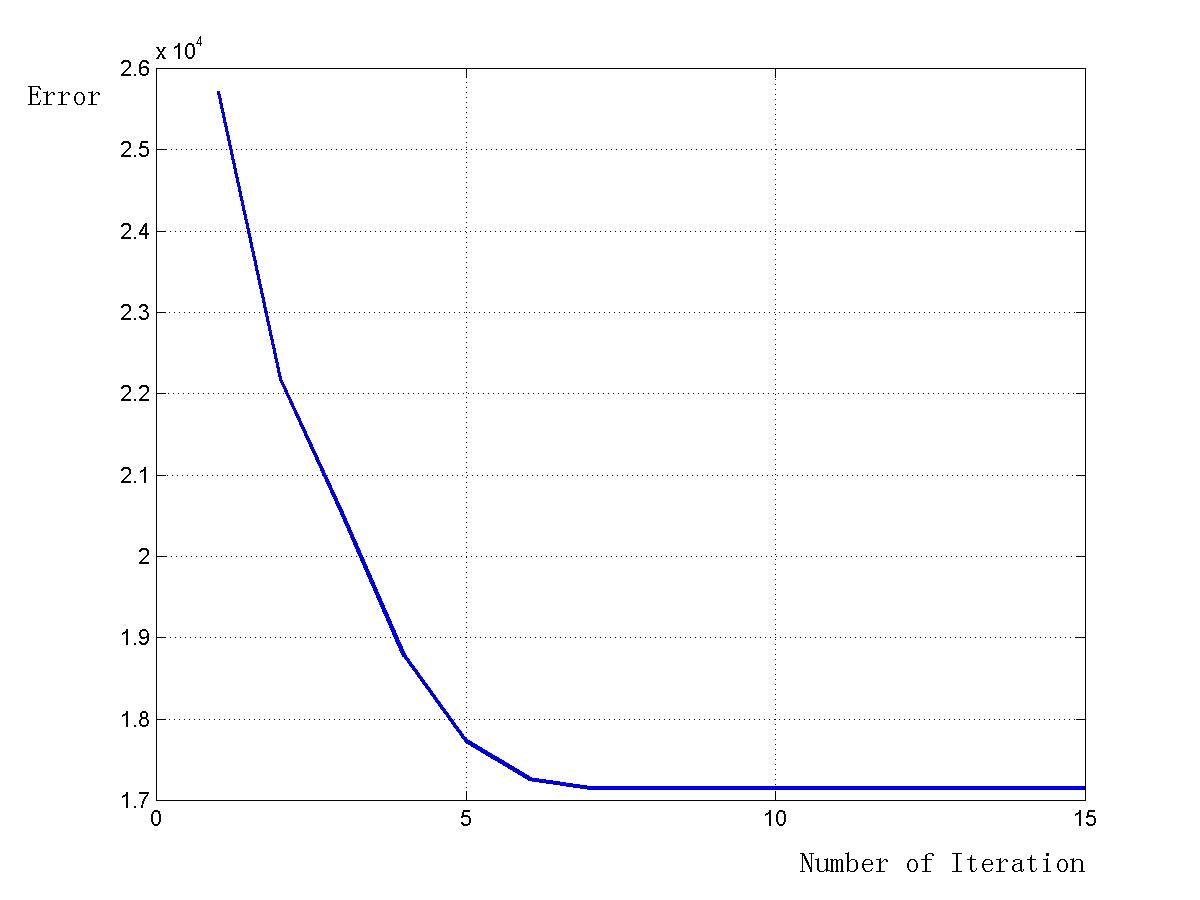
\includegraphics[width=\columnwidth]{ch3/figures/kmeanserror.jpg}
\caption{The plot of the error convergence on a $k$-mean clustering computation.}
\label{fig:kmeanserror}
\end{figure} 

Such direct $k$-means algorithm requires time proportional to the product of the number of examples and the number of clusters. This is computationally very expensive especially for large datasets.  However, in this case, the dataset is limited to the $500$ to $1000$ examples. The direct $k$-means algorithm is still effective for the task.

\section{ORL Face Database}
In this chapter, the face database used is called ORL face database. ORL is made by AT\&T Laboratories in Cambridge. It contains a set of face images taken between April 1992 and April 1994 at the AT\&T lab. There are ten different images of each of $40$ distinct subjects making $400$ images in all. For some subjects (person), the images were taken at different times, varying the lighting, facial expressions (open / closed eyes, smiling / not smiling) and facial details (glasses / no glasses). All the images were taken against a dark homogeneous background with the subjects in an upright, frontal position (with tolerance for some side movement). The examples from four subject are shown in \mbox{Figure} \ref{fig:orl}. 
\begin{figure}[ht]
 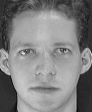
\includegraphics[width=\columnwidth/11]{ch3/figures/s1_1.png}
 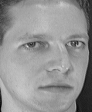
\includegraphics[width=\columnwidth/11]{ch3/figures/s1_2.png}
 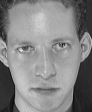
\includegraphics[width=\columnwidth/11]{ch3/figures/s1_3.png}
 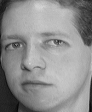
\includegraphics[width=\columnwidth/11]{ch3/figures/s1_4.png}
 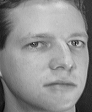
\includegraphics[width=\columnwidth/11]{ch3/figures/s1_5.png}
 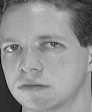
\includegraphics[width=\columnwidth/11]{ch3/figures/s1_6.png}
 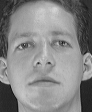
\includegraphics[width=\columnwidth/11]{ch3/figures/s1_7.png}
 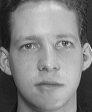
\includegraphics[width=\columnwidth/11]{ch3/figures/s1_8.png}
 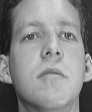
\includegraphics[width=\columnwidth/11]{ch3/figures/s1_9.png}
 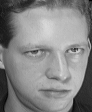
\includegraphics[width=\columnwidth/11]{ch3/figures/s1_10.png}\\
 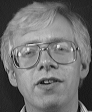
\includegraphics[width=\columnwidth/11]{ch3/figures/s2_1.png}
 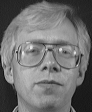
\includegraphics[width=\columnwidth/11]{ch3/figures/s2_2.png}
 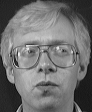
\includegraphics[width=\columnwidth/11]{ch3/figures/s2_3.png}
 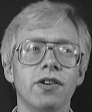
\includegraphics[width=\columnwidth/11]{ch3/figures/s2_4.png}
 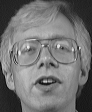
\includegraphics[width=\columnwidth/11]{ch3/figures/s2_5.png}
 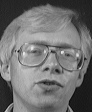
\includegraphics[width=\columnwidth/11]{ch3/figures/s2_6.png}
 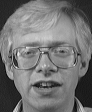
\includegraphics[width=\columnwidth/11]{ch3/figures/s2_7.png}
 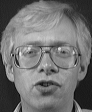
\includegraphics[width=\columnwidth/11]{ch3/figures/s2_8.png}
 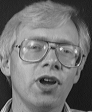
\includegraphics[width=\columnwidth/11]{ch3/figures/s2_9.png}
 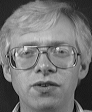
\includegraphics[width=\columnwidth/11]{ch3/figures/s2_10.png}\\
 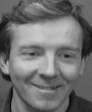
\includegraphics[width=\columnwidth/11]{ch3/figures/s3_1.png}
 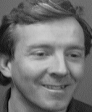
\includegraphics[width=\columnwidth/11]{ch3/figures/s3_2.png}
 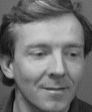
\includegraphics[width=\columnwidth/11]{ch3/figures/s3_3.png}
 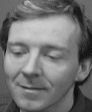
\includegraphics[width=\columnwidth/11]{ch3/figures/s3_4.png}
 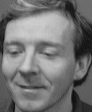
\includegraphics[width=\columnwidth/11]{ch3/figures/s3_5.png}
 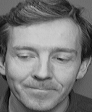
\includegraphics[width=\columnwidth/11]{ch3/figures/s3_6.png}
 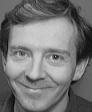
\includegraphics[width=\columnwidth/11]{ch3/figures/s3_7.png}
 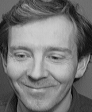
\includegraphics[width=\columnwidth/11]{ch3/figures/s3_8.png}
 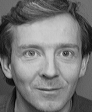
\includegraphics[width=\columnwidth/11]{ch3/figures/s3_9.png}
 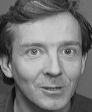
\includegraphics[width=\columnwidth/11]{ch3/figures/s3_10.png}\\
 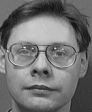
\includegraphics[width=\columnwidth/11]{ch3/figures/s4_1.png}
 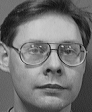
\includegraphics[width=\columnwidth/11]{ch3/figures/s4_2.png}
 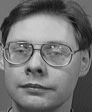
\includegraphics[width=\columnwidth/11]{ch3/figures/s4_3.png}
 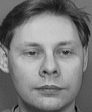
\includegraphics[width=\columnwidth/11]{ch3/figures/s4_4.png}
 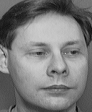
\includegraphics[width=\columnwidth/11]{ch3/figures/s4_5.png}
 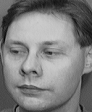
\includegraphics[width=\columnwidth/11]{ch3/figures/s4_6.png}
 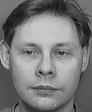
\includegraphics[width=\columnwidth/11]{ch3/figures/s4_7.png}
 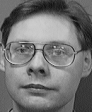
\includegraphics[width=\columnwidth/11]{ch3/figures/s4_8.png}
 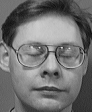
\includegraphics[width=\columnwidth/11]{ch3/figures/s4_9.png}
 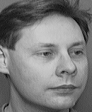
\includegraphics[width=\columnwidth/11]{ch3/figures/s4_10.png}\\
 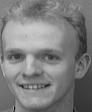
\includegraphics[width=\columnwidth/11]{ch3/figures/s5_1.png}
 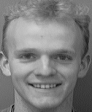
\includegraphics[width=\columnwidth/11]{ch3/figures/s5_2.png}
 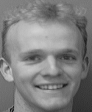
\includegraphics[width=\columnwidth/11]{ch3/figures/s5_3.png}
 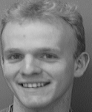
\includegraphics[width=\columnwidth/11]{ch3/figures/s5_4.png}
 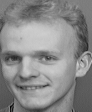
\includegraphics[width=\columnwidth/11]{ch3/figures/s5_5.png}
 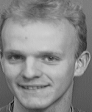
\includegraphics[width=\columnwidth/11]{ch3/figures/s5_6.png}
 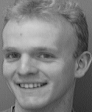
\includegraphics[width=\columnwidth/11]{ch3/figures/s5_7.png}
 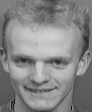
\includegraphics[width=\columnwidth/11]{ch3/figures/s5_8.png}
 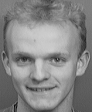
\includegraphics[width=\columnwidth/11]{ch3/figures/s5_9.png}
 \includegraphics[width=\columnwidth/11]{ch3/figures/s5_10.png}\\
 \includegraphics[width=\columnwidth/11]{ch3/figures/s6_1.png}
 \includegraphics[width=\columnwidth/11]{ch3/figures/s6_2.png}
 \includegraphics[width=\columnwidth/11]{ch3/figures/s6_3.png}
 \includegraphics[width=\columnwidth/11]{ch3/figures/s6_4.png}
 \includegraphics[width=\columnwidth/11]{ch3/figures/s6_5.png}
 \includegraphics[width=\columnwidth/11]{ch3/figures/s6_6.png}
 \includegraphics[width=\columnwidth/11]{ch3/figures/s6_7.png}
 \includegraphics[width=\columnwidth/11]{ch3/figures/s6_8.png}
 \includegraphics[width=\columnwidth/11]{ch3/figures/s6_9.png}
 \includegraphics[width=\columnwidth/11]{ch3/figures/s6_10.png}\\
\caption{The images from the ORL face database}
\label{fig:orl}
\end{figure} 
Each subject has ten different images. Some subjects are wearing glasses, but some are not. Even in one subject, some images contain the glasses, but some are not. The size of each image is $92\times 112$ pixels, with $256$ grey levels per pixel. 

\subsection{Feature Localisation Algorithm}
In face recognition, some intuitional facial features ,such as eyes, nose, lips and etc, are very important for the recognition purposes, because computer vision is an analog to human visual perception. Some general approaches for object-recognition like Principle Component Analysis (PCA) \cite{Turk1991} extract the global features, like the overall shape of the heads. For these approaches, it is hard to extract local facial features. In the chapter, local facial features are extracted rather than using the general approaches such as PCA, because human face is a particular object for recognition, the general approaches are designed to deal with the general objects rather than the particular objects. Human face is such a particular object, so that a particular approach is needed for it. In face recognition, some facial features are added to the general approaches. Facial features can not be ignored, because they are some important parts for the object model. In building face models, it is necessary to build such a model with the eyes, the nose, the nose's holes, lips, or the corners of mouth. 

Gabor filters and $k$-means clustering approach are used to find the significant facial features on the faces. When these features are projected back to the original face images, the features are identical to the eyes, nostrils and lips. The method can be used for semi-automatic locating human facial features, due to the implementation of arbitrary manual segmentation. However, the method could be fast and reliable for facial feature localisation, if some automatic segmentation of human facial area can be adopted. 

In this section, a modified Gabor for the experiment is introduced. The magnitude response is used for the later clustering process. Some pre-processing  before the direct implementation of clustering algorithm is presented.

\subsubsection{Modified Gabors}
First of all, Gabor filters are suitable for extracting some facial information. It is necessary that the Gabor filters are modified, so that they can extract some information relevant to human faces. The Gabor filter can be modeled as,
\begin{equation}
 h(x,y,\sigma,U,V)=\frac{1}{2\pi\sigma^2}\exp\{-\frac{x^2+y^2}{2\sigma^2}\}\exp[j2\pi(Ux+Vy)]
\end{equation}
so that the Gabor becomes a five-parameter function. The parameters $x$ and $y$ are the Cartesian coordinates in the image. In a template, these two parameters become the horizontal and vertical coordinates of the template windows. The parameter $\sigma$ is the standard deviation of Gaussian along $x$ and $y$. It also can be defined as the covariance matrix $ \mathbf{C} = \left( \begin{array}{cc}
             \sigma_x^2 & 0 \\
	     0 & \sigma_y^2 \\
            \end{array} \right)$. 
The parameters $U$ and $V$ are the spatial frequencies of the filter in the frequency domain along $x$ and $y$. The Gabor filters are fitted in squared $n\times n$ ($n$ is an odd) templates, such as $7\times 7$, $13\times 13$, $19\times 19$ or etc. The coordinates $x$ and $y$ are in the range of $[-\frac{n-1}{2},\frac{n-1}{2}]$. The coordinate of the origin of the template windows is $(0,0)$. In this way, the values of $x$ and $y$ are specified.

Three parameters $\sigma$, $U$ and $V$ are needed to specified. It is known that the radial frequency $F=\sqrt{U^2+V^2}$, also the spatial frequencies $U$ and $V$ of the filter is related to the rotation angle $\theta$ of the modulating Gaussian by $U=F\times \cos\theta$ and $V=F\times \sin\theta$. A constraint which is from the some physiological findings \cite{Daugman1985, Lee1996} is introduced. The constraint describes as
\begin{quotation}
The half-amplitude bandwidth of the frequency response is about 1 to 1.5 octaves along the optimal orientations. \cite{Lee1996}
\end{quotation} 
The relationship between the parameters $\sigma$ and $F$ can be derived from \cite{Lee1996} is
\begin{equation}
 \sigma = \frac{\kappa}{F} \qquad \textrm{where}\quad \kappa=\sqrt{2\ln2}(\frac{2^\varphi+1}{2^\varphi-1})
\end{equation}
where $\varphi$ us the bandwidth in octaves. For $\varphi$ in one octave, $\sigma=\frac{\pi}{F}$. For $\varphi$ in 1.5 octave, $\sigma=\frac{2.5}{F}$. If the orientation $\theta$ of Gabor filter and the standard derivation of 2D Gaussian are specified, the spatial frequencies $U$ and $V$ are
\begin{displaymath}
 \begin{array}{lll}
  U=\frac{\pi}{\sigma}\cos\theta & \textrm{and}\quad V=\frac{\pi}{\sigma}\sin\theta & \textrm{when} \quad \varphi = 1\, \mathrm{octave} \\
  U=\frac{2.5}{\sigma}\cos\theta & \textrm{and}\quad V=\frac{2.5}{\sigma}\sin\theta & \textrm{when} \quad \varphi = 1.5\, \mathrm{octave} 
 \end{array}
\end{displaymath}
In this way, the spatial frequencies are determined. In the chapter, the bandwidth is chosen as $1.0$ octave \footnote{However, some evidence \cite{Lee1996} shows that $1.5$ octave is a better choice.}

As mentioned before, the face images are convolved with the Gabor functions. In the approach of image processing, the Gabor filters are formed in the templates. The size of squared patches are required to be odd number. Since the 2D Gabor function is a product of a Gaussian and a complex plane wave, the size of Gaussian is required to determine. Dunn and Higgins \cite{Dunn1995} proposed that Gabor filters were truncated to a width of $6\sigma+1$ points, which can produce filters having a wide spatial extent (e.g., if $\sigma = 24$ pixels, filter size is $145\times 145$). Because they use the Gabor filters for the texture segmentation, texture image is quite large in the size of $512\times 512$, so that such large filters can be applied. In face recognition, the size of face image is $92\times 112$ pixels, which are from the \mbox{ORL} face database. It is required that the size of Gabor filters are kept smaller. Eight different scales of Gabor filter are considered. Their standard deviations $\sigma$ of 2D Gaussian are $1$, $2$, $3$, $4$, $5$, $6$, $7$, $8$ according to the spatial extent $7\times 7$, $13\times 13$, $19\times 19$, $25\times 25$, $31\times 31$, $37\times 37$, $43\times 43$, $49\times 49$. Examples of Gabor filter templates are given in \mbox{Figure} \ref{fig:examplesofGaborfilter}.
\begin{figure}[ht]
\begin{center}
 \subfigure[The real part in 2D plot]{\includegraphics[width=0.2\columnwidth]{ch3/figures/realpart2d.png}}
 \subfigure[The imaginary part in 2D plot]{\includegraphics[width=0.2\columnwidth]{ch3/figures/imagpart2d.png}}\\
 \subfigure[The real part in 3D mesh plot]{\includegraphics[width=0.48\columnwidth]{ch3/figures/realpart3d.png}}
 \subfigure[The imaginary part in 3D mesh plot]{\includegraphics[width=0.48\columnwidth]{ch3/figures/imagpart3d.png}}\\
\caption{The example of Gabor filter with the standard deviation $\sigma=8$, the orientation $\theta=\frac{\pi}{4}$, and the bandwidth $\varphi=1.0$}
\label{fig:examplesofGaborfilter}
\end{center}
\end{figure} 

Also four orientations are specified, which are $\theta=\{-\pi/4, 0,\pi/4, \pi/2 \}$. So the whole bunch of filters is shown in \mbox{Figure} \ref{fig:allgabors}.
\begin{figure}[ht]
 \includegraphics[width=\columnwidth]{ch3/figures/allgabors.png}
\caption{The whole filters in 8 different scales and 4 different orientations}
\label{fig:allgabors}
\end{figure} 
From the top to the bottom, the derivation $\sigma$ of Gabor increases by 1 pixel from 1 to 8. From the left to the right, the orientation changes in $0$, $\pi/4$, $\pi/2$, $-\pi/4$. The left four columns are the real parts of filters, and the right four columns are the imaginary parts.

\subsubsection{The magnitude response}
The odd and even responses give the results in which the pixel value is varied from negative to position. The magnitude responses give results in which the pixel value is only in positive or zero. If the Gabor filters to the face image are applied, the pixels' values in responses range very widely from the very high  $40.2398$ to low $5.4026e^{-4}$. In facial analysis, it is only concern about the high response which may be some crucial facial features like eyes, nose holes, lips and etc, but the low responses represent some smooth varying area on the face, like cheek. For the objectives which are to model the face, the high response from the facial feature area is used, but the low responses from other areas on the face are ignored.

Only the magnitude responses is used in the thesis. The reason is that, the magnitude response contains both information in real one and imaginary one. The real and imaginary responses give the results both in positive and negative. For image processing, the magnitude response is easy to deal with. For instance, when Gabor filters are applied in the edge detection, the real and imaginary response to the changing area in an image is difficult to give any meaningful interpretation. If the magnitude responses are applied in edge detection, the responses give results indicating the edge. The same results are obtained both from texture detection and segmentation. 
It is possible that the magnitude responses may lose some information because it only use the the squared sum. Other important factor - phase response has been ignored for the implementation, but the phase responses indicate some meaningful information when applied on face images, as it described in \mbox{Figure} \ref{fig:magandphase}. So the only magnitude response is not a good solution for the face recognition purpose.
\begin{figure}[ht]
\begin{center}
 \subfigure{\includegraphics[width=0.15\columnwidth]{ch3/figures/originface.png}}
 \subfigure{\includegraphics[width=0.15\columnwidth]{ch3/figures/magpartface.png}}
 \subfigure{\includegraphics[width=0.15\columnwidth]{ch3/figures/phasepartface.png}}
\caption{The original face image, the magnitude response, and the phase response}
\label{fig:magandphase}
\end{center}
\end{figure} 

When the size of the template is small, the responses will capture more detailed changes in images. In responses, some facial features are clear to recognise by human visual perception system. However, when the size of template (also the derivation of Gaussian) increases, the responses become more rough, as shown in \mbox{Figure} \ref{fig:multimagreponse}.
\begin{figure}[ht]
\begin{center}
 \subfigure{\includegraphics[width=0.15\columnwidth]{ch3/figures/originface.png}}
 \subfigure[$\sigma=1$]{\includegraphics[width=0.15\columnwidth]{ch3/figures/magresponse1.png}}
 \subfigure[$\sigma=4$]{\includegraphics[width=0.15\columnwidth]{ch3/figures/magresponse2.png}}
 \subfigure[$\sigma=8$]{\includegraphics[width=0.15\columnwidth]{ch3/figures/magresponse3.png}}
\caption{The original face image with multiple magnitude responses}
\label{fig:multimagreponse}
\end{center}
\end{figure} 
The magnitude responses from the filter with the standard derivation $\sigma=1$, $\sigma=4$, $\sigma=8$ are shown. When the standard derivation is small, the eyes and nostrils are clear. When the derivation becomes higher i.e. $\sigma=4$, the responses on these areas become more rough, but still can be recognised. When the derivation becomes the highest ($\sigma=8$ ), the responses become the most rough, and some different features, which also give the insight of selection of filters, are not distinguished.

\subsubsection{Preparing for the clustering}
Among these four different orientations, when $\theta=\pi/2$, the Gabor filtering on face images gets more response on face features’ areas, because this Gabor captures the changes in the vertical direction, which likes the bars in the horizontal direction, and most facial features are laid in the horizontal direction. So the horizontal Gabor filter is adopted. The single Gabor scheme is used rather than the bank of Gabor filters or Gabor wavelets. The smallest Gabor filter having $\sigma=1$ is used, because the Gabor gives the finest responses. The result of this Gabor applied on the face image is shown in \mbox{Figure} \ref{fig:smallestgaborresult}.
\begin{figure}[ht]
 \begin{center}
  \subfigure{\includegraphics[width=0.15\columnwidth]{ch3/figures/originface.png}}
  \subfigure{\includegraphics[width=0.15\columnwidth]{ch3/figures/magresponseA.png}}
  \caption{The magnitude response of face image convolved with the Gabor filter with the parameters $\sigma=1$, $\varphi=1.0$ and $\theta=\pi/2$}
  \label{fig:smallestgaborresult}
 \end{center} 
\end{figure}
An interested phenomenon is discovered in this figure. The responses in the area of two eyes, nose and mouth resemble four clusters of bright points if the strong points of responses are neglected. From the phenomenon, it is supposed that some clustering algorithm can be used on these responses to get the features. 

Before the clustering algorithm is used, some preprocesses are applied on the response images. First of all, the facial part excluding the hair and the ears is the only interesting area. In the response image, the areas where the hair and ears locate also give strong responses. Those responses are useless for the face recognition purpose (but in human face detection the hairline is an important clue), because the inner facial part is only concerned. The segmentation on face images is performed manually. A rectangle image is extracted from the original response image. The segmented inner face parts only contain the two eyes, nose and mouth. However, the manual method involves the humans' intervention because different face has various features locating on different locations. \mbox{Figure} \ref{fig:3dMag} is this segmented image on a 3D mesh with small hills on those areas.
\begin{figure}[ht]
\begin{center}
  \includegraphics[width=\columnwidth]{ch3/figures/3dMagtitude.png}
\caption{The 3D mesh plot of a segmented image contains facial part.}
\label{fig:3dMag}
\end{center}
\end{figure} 
The two ``peaks'' are corresponding to two eyes. The two long ``mountains'' are corresponding to the nose and the mouth. In other areas, there are some small ``hills'', which need to be removed by using a threshold.

A threshold is chosen to remove the weak responses. To find the threshold, the segmented images are analysed by the distribution of responses. \mbox{Figure} \ref{fig:segmentimagehisto} shows the histogram of a segmented image. 
\begin{figure}[ht]
\begin{center}
 \includegraphics[width=0.66\columnwidth]{ch3/figures/segmentHisto.png}
\caption{The histogram of one segmented image and the colour bar shows the different colours indicate different values.}
\label{fig:segmentimagehisto}
\end{center}
\end{figure} 
From this graph, it is found that most responses are less than 3.2, and these are also weak responses. The responses which greater than $3.2$ will be the strong responses. In this case, the threshold is determined as $3.2$. However, such method of manually finding the threshold will vary in different images. So it is necessary to find some automatics threshold algorithms.

After these two processes, the image becomes a binary image. It also can be viewed as some points in 2D space as shown in \mbox{Figure} \ref{fig:pointson2dspace}. There may be four or five clusters in this space. 
\begin{figure}[ht]
\begin{center}
 \includegraphics[width=0.66\columnwidth]{ch3/figures/pointson2dspace.png}
\caption{The points remained after the segmentation and thresholding.}
\label{fig:pointson2dspace}
\end{center}
\end{figure} 

\subsubsection{Clustering algorithm on face images.}
For performing $k$-means clustering, the responses are explained as examples which include two coordinates in the images. The number of clusters is specified as $5$, and the $k$-means clustering is run on these example. The result is shown in \mbox{Figure} \ref{fig:kmeanspointson2dspace}.
\begin{figure}[ht]
\begin{center}
 \includegraphics[width=0.66\columnwidth]{ch3/figures/kmeanspointson2dspace.png}
\caption{Different clusters are specified with different colours after $k$-means algorithm with $k=5$.}
\label{fig:kmeanspointson2dspace}
\end{center}
\end{figure} 
The $k$-means algorithm normally takes less than $12$ iterations before the error ceases to vary significantly. In this figure, the algorithm automatically locates five clusters. These five clusters are around two eyes, nostrils, and left and right part of lips. The different clusters are represented by different colours. The enters of clusters are represented by the small red circles.

\subsection{Results}
The $k$-means algorithm applied on the face image shows some significant rates and results. The reason is those clusters are separated distinguishably. There are some distinct clusters in different areas. And the algorithm normally runs $8\sim 12$ iterations. It will not take long time to compute. The $k$-means algorithm is capable for the task of automatic locating some significant facial features. 

To compare the features that this approach captured with the facial features that already exist in the human faces, the centroids of these clusters are projected back to the original face images. These five points are identical to two eyes, the bottom of the bridge of nose, and one point in the right part of mouth and one point in the left part. Some examples are shown in \mbox{Figure} \ref{fig:fivepointsnormal}. 
\begin{figure}[ht]
\begin{center}
 \includegraphics[width=0.15\columnwidth]{ch3/figures/kmeanresult1.png}
 \includegraphics[width=0.15\columnwidth]{ch3/figures/kmeanresult2.png}
 \includegraphics[width=0.15\columnwidth]{ch3/figures/kmeanresult3.png}
 \includegraphics[width=0.15\columnwidth]{ch3/figures/kmeanresult4.png}
 \includegraphics[width=0.15\columnwidth]{ch3/figures/kmeanresult5.png}\\
 \includegraphics[width=0.15\columnwidth]{ch3/figures/kmeanresult6.png}
 \includegraphics[width=0.15\columnwidth]{ch3/figures/kmeanresult7.png}
 \includegraphics[width=0.15\columnwidth]{ch3/figures/kmeanresult8.png}
 \includegraphics[width=0.15\columnwidth]{ch3/figures/kmeanresult9.png}
 \includegraphics[width=0.15\columnwidth]{ch3/figures/kmeanresult10.png}\\
 \includegraphics[width=0.15\columnwidth]{ch3/figures/kmeanresult11.png}
 \includegraphics[width=0.15\columnwidth]{ch3/figures/kmeanresult12.png}
 \includegraphics[width=0.15\columnwidth]{ch3/figures/kmeanresult13.png}
 \includegraphics[width=0.15\columnwidth]{ch3/figures/kmeanresult14.png}
 \includegraphics[width=0.15\columnwidth]{ch3/figures/kmeanresult15.png}\\
 \includegraphics[width=0.15\columnwidth]{ch3/figures/kmeanresult16.png}
 \includegraphics[width=0.15\columnwidth]{ch3/figures/kmeanresult17.png}
 \includegraphics[width=0.15\columnwidth]{ch3/figures/kmeanresult18.png}
 \includegraphics[width=0.15\columnwidth]{ch3/figures/kmeanresult19.png}
 \includegraphics[width=0.15\columnwidth]{ch3/figures/kmeanresult20.png}
\caption{The centroids of five clusters (corresponding to two eyes, bottom of nose and mouth) are projected back to the original face images after the $k$-means clustering}
\label{fig:fivepointsnormal}
\end{center}
\end{figure} 
Although some points on the images vary, these points are still around these facial features. Obviously, the approach is robust to the subject that has beard or mustache.

However, on some face images, this algorithm fails, or it can be explained that the other kinds of features the algorithm will capture. These faces are special, because the subjects are wearing glasses. However, this five-point strategy captures other features. Two points are still identical to the two eyes, but one point locates in the middle of mouth and the rest two points appear on the bottom edge of the glass. This finding may help to model the glasses. Some example shows in \mbox{Figure} \ref{fig:withglasses}.
\begin{figure}[ht]
 \begin{center}
  \includegraphics[width=0.15\columnwidth]{ch3/figures/badglass1.png}
  \includegraphics[width=0.15\columnwidth]{ch3/figures/badglass2.png}
  \includegraphics[width=0.15\columnwidth]{ch3/figures/badglass3.png}
  \includegraphics[width=0.15\columnwidth]{ch3/figures/badglass4.png}
  \includegraphics[width=0.15\columnwidth]{ch3/figures/badglass5.png}\\
  \includegraphics[width=0.15\columnwidth]{ch3/figures/badglass6.png}
  \includegraphics[width=0.15\columnwidth]{ch3/figures/badglass7.png}
  \includegraphics[width=0.15\columnwidth]{ch3/figures/badglass8.png}
  \includegraphics[width=0.15\columnwidth]{ch3/figures/badglass9.png}
  \includegraphics[width=0.15\columnwidth]{ch3/figures/badglass10.png}
\caption{The results of this five-point strategy applied on some special face images in which the subjects wear the glasses.}
\label{fig:withglasses}
 \end{center}
\end{figure} 
It shows two points appear on the bottom of glasses. The last subject has no glass, but her eyebrows and wrinkles below the eyes are very clear, which make her look like wearing glasses. 

No matter which kind of subjects, non-glass or wearing glasses are dealt with. The approach still can capture the features such as eyes and mouth. For a subject who is not wearing glasses, this five-point strategy is capable. This approach is quite successful for locating some significant facial features on faces. 
\subsection{Discussion}
A semi-automatic approach of locating the facial features is proposed. In the approach, firstly the Gabor filter was used for extracting the necessary facial information, and then the $k$-means clustering algorithm is applied on this information which is in the form of two-dimensional examples. The results show that this approach is capable of finding the locations of facial features. The approach at least can capture the eyes and mouth, and also other locations depending on whether the subject is wearing glasses or not. The approach shows its success on the ORL face database.

However, there are two parts which are operated manually. One is the rectangle after the segmentation of the face images. A rectangle is chosen with the best size and position. The rectangles of face images contain the features of eyes, nose and mouth, but not include the hair, the ears and the background.  The new approach should have a rectangle or ellipse contains those features as happened in some face detection. The other one is the threshold for removing some small responses. The threshold is chosen manually after an analysis of histogram of the response image. It is assumed that most areas have the weak responses, and some facial areas have the strong responses. The threshold of weak responses is estimated empirically. An automatics thresholding algorithm, such as Otsu thresholding can be used to overcome the shortage.

This approach only uses one Gabor filter. However, one Gabor only extracts part of information, and loss some other information. More Gabors should be used to form a filter bank or to generate the Gabor Wavelets. Also the parameters in Gabors are hardly to be specified. This approach only chooses some arbitrary values of the parameters. It leaves a question on whether these parameters are suitable for face recognition purpose. The optimal solution for the parameters is needed. The wavelets are competent for the task, because we can use the wavelets to reconstruct the original images. By minimising the difference between the original one and the reconstructed one, the problem of optimal parameters can be fixed \cite{Lee1996}.  In the latter work, the Gabor wavelet will be used for the feature extracting.

\chapter{Extended Gabor-based method}
The above approach only uses one Gabor filter. From the point view of wavelets, single channel is not enough to describe the features. Therefore, a multi-channel scheme was adopted to improve the performance of facial features localisation. The work was motivated by Jain and Farrokhnia’s work \cite{Jain1991} on unsupervised texture segmentation. They presented a texture segmentation algorithm inspired by the multi-channel filtering theory for visual information processing in the early stages of human visual system. The channels are described by a bank of Gabor filters that uniformly cover the spatial-frequency domain. A filter selection scheme is proposed, which is based on reconstruction of the input image from the filtered images. Texture features are obtained by submitting each filtered image to a nonlinear transformation and computing a measure of ``energy'' in a window around each pixel. A square-error clustering algorithm is then used to integrate the feature images and produce a segmentation.
\section{Texture Segmentation}
Human face as a specified object also contains textures. Skin can be considered as one  texture, and hairs can be taken as other textures, the background of face image (if it is unique) also is one kind of textures, so as to lips, eyes. Therefore, the Gabor filter based texture segmentation can be used in localising the facial features. 

An important issue in the multi-channel filtering approach to texture analysis is the characterisation of the channels. The representation uses real-valued, even-symmetric Gabor filters. The impulse response of an even-symmetric Gabor filter is given by
\begin{equation}
 h(x,y)=\exp\{-\frac{1}{2} [\frac{x^2}{\sigma_x^2}+\frac{y^2}{\sigma_y^2}] \} \cos(2\pi u_0 x)
\end{equation}
where $u_0$ is the frequency of a sinusoidal plane wave along the $x$-axis. The parameters $\sigma_x$ and $\sigma_y$ are the space constants of the Gaussian envelope along the $x$ and $y$ axes respectively. Filters with arbitrary orientations can be obtained via a rigid rotation of the $x-y$ coordinates. In addition to the radial frequency and the orientation, the frequency bandwidth $B_T$ and the orientation bandwidth $B_{\theta}$ of filter are also taken into account. There are four values of orientation $\theta_0$ used: $0$, $\pi/4$, $\pi/2$, and $3\pi/4$. The finer quantisation of orientation may be needed in general purpose of computer vision application. However, the restriction to these four orientations is made for computational efficiency, and is sufficient for discriminating many textures. For an image with a width of $N_c$ pixels, where $N_c$ is a power of $2$ (so that the size of image is in even numbers), the following values of radial frequency $u_0$ are used:
\begin{displaymath}
2^n \sqrt{2} \quad \textrm{where} n = \{0,1,\ldots\}
\end{displaymath}
and
\begin{displaymath}
 \frac{N_c}{4}\sqrt{2} \quad \textrm{cycles image-width}^{-1}
\end{displaymath}
The total number of Gabor filters in the filter set is given by $4\log_2(\frac{N_c}{2})$. For an image with $256$ pixel-width, for example, a total of $28$ filters can be used $4$ orientations and $7$ radial frequencies. However, for some textures,filters with low radial frequencies are not very useful, because these filters capture spatial variations that are too large to explain textural variations in an image.

The systematic filter selection scheme is based on an intuitive least squares error criterion. Using only a subset of the filtered images can reduce the computational burden at later stages, because this directly translates into a reduction in the number of texture features. The reconstruction $s(x, y)$ of the input image is obtained by adding all the filtered images. It is assumed that $s(x, y)$ is the best approximation of the original image. Then $\hat{s}(x,y)$ is the partial reconstruction of the image obtained by adding a given subset of filtered images. The error involved in using $\hat{s}(x,y)$ instead of $s(x, y)$ can be measured by 
\begin{equation}
 SSE = \sum_{x,y}[\hat{s}(x,y)-s(x, y)]^2
\end{equation}
The fraction of intensity variations in $s(x, y)$ that is explained by $\hat{s}(x,y)$ can be measured by coefficient of determination (COD)
\begin{equation}
 R^2=1-\frac{SSE}{SSTOT} \qquad \textrm{where} \quad SSTOT = \sum_{x,y}[s(x,y)]^2
\end{equation}

The bigger the $R^2$ (COD) is, the best subset of filtered images is selected. Note that $s(x, y)$ has a mean of zero, since the mean grey value of each filtered image is zero. The filter selection scheme is to use only a subset of filtered images that forms a optimal portion of the intensity variations in $s(x, y)$. The best subset of the filtered images is determined by the following sequential forward selection procedure. The procedure is described in \mbox{Table} \ref{tab:sfsp}.
\begin{table}[ht]
 \begin{algorithmic}[1]
  \STATE select the filtered image that best approximates $s(x, y)$, i.e. results in the highest value of $R^2$;
  \STATE select the next filtered image that together with previously selected filtered images best approximate $s(x, y)$;
  \STATE repeat step 2 until $R^2\ge 0.99$
 \end{algorithmic}

\caption{The sequential forward selection procedure}
\label{tab:sfsp}
\end{table} 

For computing features from each filtered image, first each filtered image is subjected to a nonlinear transformation. Specifically, the following bounded nonlinearity
\begin{equation}
 \Psi(t)=\tanh(\alpha t)=\frac{1-e^{-2\alpha t}}{1+e^{-2\alpha t}}
\end{equation}
Here, an empirical value $\alpha=0.25$ is used. Formally, the feature image $e_k(x, y)$ corresponding to filtered image $r_k(x, y)$ is given by
\begin{equation}
 e_k(x,y)=\frac{1}{M^2}\sum_{(a,b)\in W_{xy}} \|\Psi(r_k(a,b))\|
\end{equation}
where $\Psi()$ is the nonlinear function and $W_xy$ is an $M\times M$ window centred at the pixel with coordinates $(x, y)$.

Having obtained the feature images, the main question is how to integrate features corresponding to different filters to produce a segmentation. Again the $k$-means algorithm was adopted. 
\section{Results}
In results, the textures on the human faces were segmented by the proposed algorithm. A small subset of Gabor filters was selected. The number of the subset is $8$. They are varied with the derivation $\sigma$ of Gaussian, frequency $f$ and orientation $\theta$. \mbox{Table} \ref{tab:detailsubsetgabor} shows the details of parametrised these Gabor filters. 
\begin{table}[ht]
\begin{center}
 \begin{tabular}{|c|c|c||c|c|c|}
 \hline
$\sigma$ & $f$ & $\theta$ & $\sigma$ & $f$ & $\theta$ \\
 \hline
$\sqrt{2}$ & $2\sqrt{2}$ & $0$ & $2\sqrt{2}$ & $5\sqrt{2}$ & $0$ \\
$\sqrt{2}$ & $3\sqrt{2}$ & $0$ & $3\sqrt{2}$ & $5\sqrt{2}$ & $0$ \\
$\sqrt{2}$ & $3\sqrt{2}$ & $\pi/2$ & $4\sqrt{2}$ & $5\sqrt{2}$ & $0$ \\
$\sqrt{2}$ & $4\sqrt{2}$ & $\pi/4$ & $\sqrt{2}$ & $5\sqrt{2}$ & $0$ \\
 \hline
 \end{tabular} 
\caption{The detail of subset of Gabor filters}
\label{tab:detailsubsetgabor}
\end{center}
\end{table} 
These Gabor filters form a filter bank. The k-means algorithm has been used on the response images with different number of clusters estimated from $3$ to $8$. Additionally, these response images were blurred by using Gaussian kernel with different size in $1$, $5$, and $10$ pixels. The results of face segmentation are shown in \mbox{Figure} \ref{fig:segmentfacegabor}.
\begin{figure}[ht]
 \begin{center}
  \includegraphics[width=\columnwidth]{ch3/figures/facesegmentgabor.png}
\caption{The results of Texture segmentation approach used on human face for localising the facial features.}
\label{fig:segmentfacegabor}
 \end{center}
\end{figure} 
In this Figure, the facial textures are well segmented. When the pre-defined number of textures is small ($k = 3$), the facial skin texture is segmented, also the background as one segmented texture. When the number of textures becomes higher ($k>6$), the results show more precise segmentation on eyes, cheek, mouth, etc. From the results, the proposed method can be used in facial texture segmentation, and the features have been allocated. The method also provides a way to detect human skin in grey-level images.